\section{Theorie}
\label{sec:theorie}

\subsection{Radioaktiver Zerfall von $\ce{^{137}Cs}$}
Das Isotop $\ce{^{137}Cs}$ zerfällt mit einer Halbwertswert von etwa $30$ Jahren
über einen $\beta$-Zerfall in $\ce{^{137}Ba}$. In $\SI{94.6}{\percent}$ der
Fälle läuft dieser Vorgang über einen angeregten Zustand von $\ce{^{137}Ba}$ ab.
Mit einer Wahrscheinlichkeit von $\SI{5.4}{\percent}$ führt der $\beta$-Zerfall
direkt in den Grundzustand des Barium-Kerns. Der Übergang des angeregten Kerns
in seinen Grundzustand erfolgt durch Aussendung eines Photons mit einer
charakteristischen Energie von $\SI{0.662}{\mega\electronvolt}$ bei einer
Halbwertszeit von $\SI{153}{\second}$. Die Energie des Photons entspricht dabei
der Energiedifferenz der beiden Zustände des Barium-Kerns.
Abbildung~\ref{fig:zerfallsschema} zeigt das Zerfallsschema von $\ce{^{137}Cs}$.

\begin{figure}
  \centering
  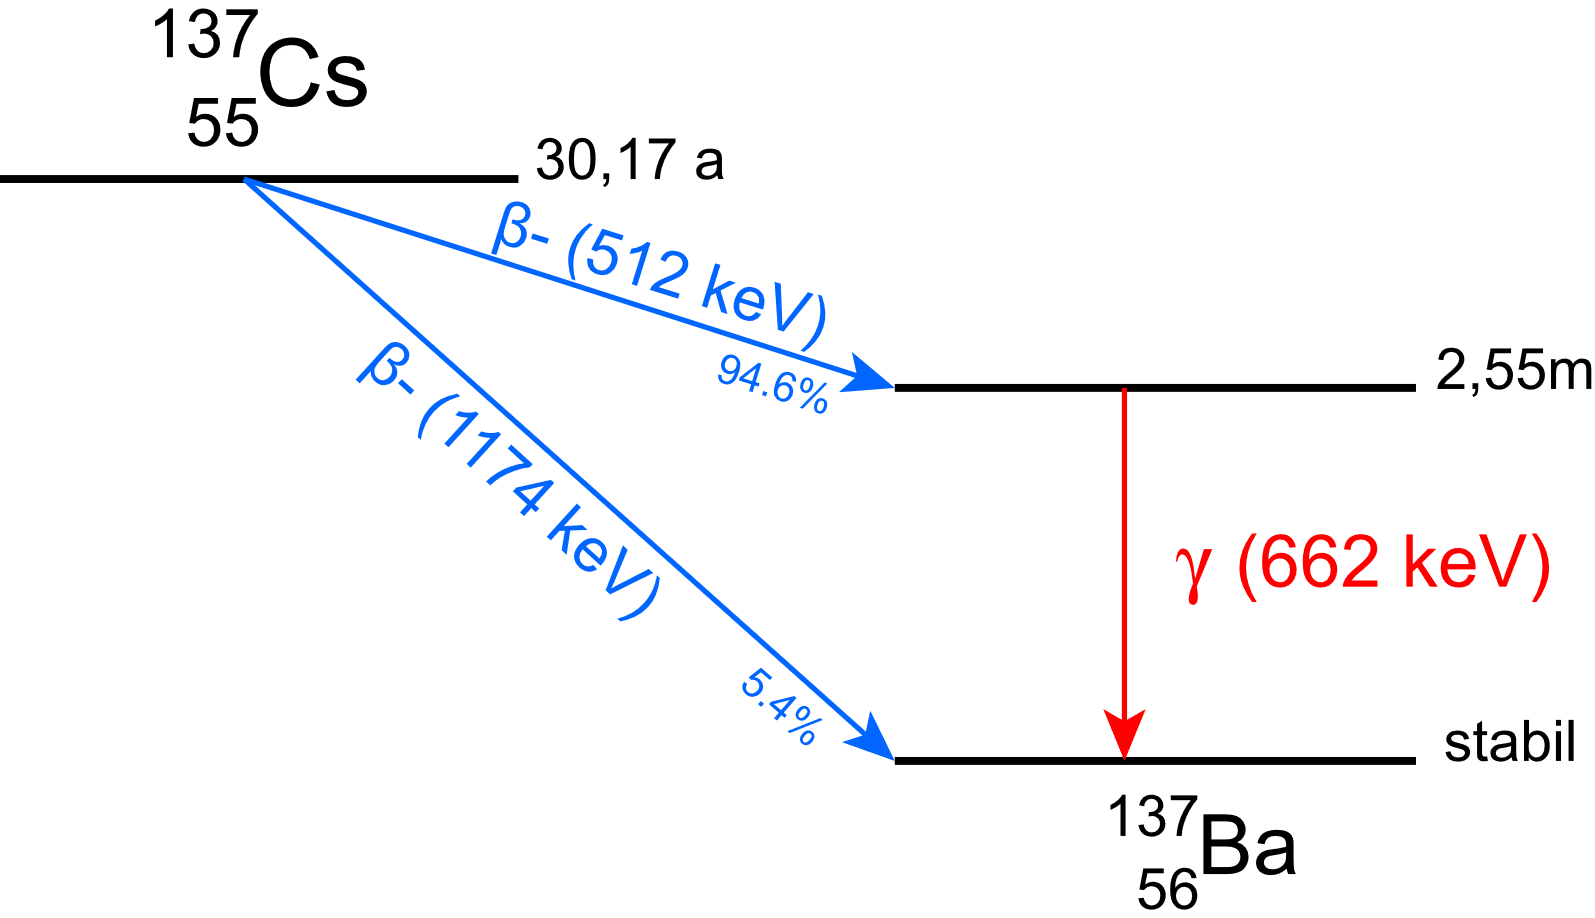
\includegraphics[width=0.75\textwidth]{figures/Cs137_Zerfallsschema.png}
  \caption{Zerfallsschema von $\ce{^{137}Cs}$ in $\ce{^{137}Ba}$. Beim Zerfall
  über einen angeregten Zustand des Barium-Kerns wird zusätzlich zum
  $\beta$-Teilchen ein $\gamma$-Quant mit der charakteristischen Energie
  $\SI{0.622}{\mega\electronvolt}$ emittiert.}
  \label{fig:zerfallsschema}
\end{figure}

\subsection{Wechselwirkung von elektromagnetischer Strahlung mit Materie}
Der Durchgang von $\gamma$-Strahlung durch Materie ist geprägt von der
Wechselwirkung der Photonen mit den Hüllenelektronen der Atome des
Absorbermaterials. Im Folgenden werden die drei in der Regel dominierenden
Prozesse diskutiert: Der Photoeffekt, die Comptonstreuung und die Paarbildung.
\begin{itemize}
  \item Der Photoeffekt beschreibt die Wechselwirkung eines Photons mit einem
  Hüllenelektron, wobei das Photon seine Energie $E_{\gamma}$ vollständig an
  das Elektron abgibt und das Elektron aus seiner Bindung  entfernt wird. Es
  erhält dabei die Energie $E_\text{e}=E_{\gamma}-E_\mathup{B}$. Das Auftreten
  des Photoeffektes erfolgt erst, sobald die Bindungsenergie $E_\mathup{B}$ des
  Elektrons kleiner als die Photonenergie ist, woraus sich die Bedingung
  $E_{\gamma}>E_\mathup{B}$ ergibt. Der Photoeffekt dominiert bei Energie unter
  $\SI{100}{\kilo\electronvolt}$. Der Wirkungsquerschnitt ist proportional zu
  $Z^5$, woraus folgt, dass der Effekt bei schweren Kernen stärker zum tragen
  kommt.
  \item Der zweite Effekt wird als Comptonstreuung bezeichnet. Hierbei wird das
  Photon an einem freien Elektron inelastisch gestreut. Das Photon gibt dabei
  unter Richtungsänderung Energie an das Elektron ab, wird dabei allerdings
  nicht vernichtet. Der Wirkungsquerschnitt der Comptonstreuung ist
  proportional zu $Z^2$. Der Effekt dominiert im Energiebereich zwischen
  $\SI{100}{\kilo\electronvolt}$ und $\SI{10}{\mega\electronvolt}$.
  \item Der dritte Prozess ist die Paarerzeugung. Sie tritt bei Energien
  oberhalb der doppelten Ruhemasse des Elektrons auf, also ab
  $\SI{1.02}{\mega\electronvolt}$. Hierbei wird der Photon unter Erzeugung eines
  Elektrons und eines Positrons ausgelöscht. Aufgrund des
  Impulserhaltungssatzes wird dabei stets auch Energie auf den Atomkern
  übertragen. Da mit $\gamma$-Strahlung der Energie
  $\SI{0.662}{\mega\electronvolt}$ gearbeitet wird, trägt die Paarerzeugung im
  folgenden Versuch nicht bei.
\end{itemize}
Durch Überlagerung der verschiedenen Effekte ergeben sich schnell komplexe
Abhängigkeiten. Stets wird ein Teil der Energie der Eingangsstrahlung im
Material absorbiert. Insgesamt folgt die Abschwächung der Eingangsintensität
$I_0$ einem expontiellen Verlauf, der Form
\begin{equation}
  I=I_0e^{-\sum_i\mu_id_i}
\end{equation}
wobei die $\mu_i$ die Absorptionskoeffizienten verschiedener Materialien und
$d_i$ deren Dicken bezeichnen. Durch Umstellen der Formel zu
\begin{equation}
  \sum_i\mu_id_i=\text{ln}\left(\frac{I_0}{I_j}\right)
  \label{eq:gls}
\end{equation}
ergibt sich die Möglichkeit durch die Messung der Intensitäten $I_j$ und bei
geschickter Wahl der Strahlwege ein Gleichungssystem aufzustellen, mit dessen
Hilfe die Verteilung verschiedener Materialien in einem nicht einsehbaren Körper
bestimmt werden kann.

\subsection{Messung der Absorptionskoeffizienten}
Im Folgenden wird mit der Matrixschreibweise gearbeitet, sodass sich
Gleichung~\eqref{eq:gls} schreiben lässt als
\begin{equation}
  A\cdot\vec{\mu}=\vec{I}
  \label{eq:gls_matrix}
\end{equation}
Hierbei bezeichnet $\vec{\mu}$ den zu bestimmenden Vektor der
Absorptionskoeffizienten, $A$ die Matrix, die Information über die Wegstrecken
enthält und $\vec{I}$ den Vektor der gemessenen Intensitäten gemäß der rechten
Seite von Gleichung~\eqref{eq:gls}.

Im durchgeführten Versuch wird ein Würfel mit dünner Aluminiumummantelung
untersucht, der im Inneren aus $3\times3\times3$ gleich großen Teilwürfel
besteht. Aus Zeitgründen wird nur eine Schicht untersucht, sodass insgesamt neun
Absorptionskoeffizienten zu bestimmen sind. Der Vektor $\vec{\mu}$ hat demnach
die Dimension $n=9$. Die Matrix $A$ hat die Dimension $m\times n$, wobei $m$ die
Dimension des Vektors $\vec{I}$, also die Anzahl der durchgeführten Messungen
bei unterschiedlichen Projektionen ist. Um das lineare Gleichungssystem mit
einem klassischen Ansatz lösen zu können, sind mindestens $n$ unterschiedliche
Projektionen zu wählen, wobei sichergestellt werden muss, dass die resultierende
Matrix $A$ nicht singulär ist. Es empfiehlt sich jedoch zu Gunsten einer
besseren Statistik mehr Messungen bzw. Projektionen durchzuführen.
Abbildung~\ref{fig:projektionen} zeigt die zwölf ausgewählten Projektionen zur
Untersuchung einer Schicht des Würfels.

Zur Berücksichtigung unterschiedlicher Unsicherheiten auf die gemessenen Werte
von $\vec{I}$ wird Gleichung~\eqref{eq:gls_matrix} modifiziert zu
\begin{equation}
  WA\cdot\vec{\mu}=W\vec{I}
\end{equation}
mit der Gewichtungsmatrix
\begin{equation}
  W=V[I]^{-1}
\end{equation}
Die Lösung der Gleichung ist nun gegeben durch
\begin{equation}
  \vec{\mu}=\left(A^TWA\right)^{-1}\left(A^TW\vec{I}\right)
\end{equation}
Für die Unsicherheiten ergibt sich
\begin{equation}
  V[\mu])\left(A^TWA\right)^{-1}
\end{equation}
